\subsection{.NET mit C\#}

C\# ist eine objektorientierte Programmiersprache, die speziell für die Entwicklung von 
Anwendungen auf der .NET-Plattform optimiert wurde. Als eine der fünf beliebtesten 
Programmiersprachen auf GitHub ist sie vollständig ``open-source''.

C\# greif die Konzepte aus JavaScript, Java und C++ auf, was sie für Leute mit Kenntnissen
in diesen Bereichen leichter zu lernen macht. Zu den zentralen Sprachmerkmalen gehören Generics, 
Pattern Matching, asynchrone Programmierung und Records. Diese Funktionen ermöglichen eine 
typsichere und strukturierte Entwicklung.

Für die Arbeit mit C\# stehen verschiedene Entwicklungsumgebungen und Werkzeuge zur Verfügung. 
Visual Studio bietet eine integrierte Entwicklungsumgebung mit umfangreichen Funktionen. 
Visual Studio Code stellt eine leichtgewichtige Alternative mit Erweiterungsmöglichkeiten 
dar. Zudem ermöglichen Kommandozeilen-Tools (CLI-Tools) eine flexible Nutzung. JetBrains Rider 
ist eine weitere IDE, die speziell für .NET optimiert wurde und in diesem Projekt
aufgrund der Erfahrung des Backend-Entwicklers genutzt wird. (siehe Kapitel \ref{subsection:jetbrains-rider})

In dieser Diplomarbeit wurde C\# für das REST-Backend verwendet. Die zentrale Datenverwaltung 
erfolgte über Entity Framework Core mit einer PostgreSQL-Datenbank. Die Authentifizierung 
wurde durch die Anbindung an Azure AD B2C mittels MSAL realisiert. REST-APIs wurden implementiert, 
um die Kommunikation mit Unity und dem Frontend zu ermöglichen. Zusätzlich wurde Azure Blob 
Storage zur Speicherung und Verwaltung von Bilddateien integriert.

Die Wahl von C\# basiert auf zwei Faktoren. Die Sprache bietet eine direkte Integration mit 
Microsoft-Diensten, einschließlich der genutzten Azure-Dienste. Zudem wird C\# im 
Programmier-Zweig der HTL-Leonding unterrichtet, sodass bereits Vorkenntnisse vorhanden 
waren, die in der Diplomarbeit genutzt werden konnten.
\footnote{Alle Informationen zu C\# stammen von: \cite{MicrosoftCorporationo}}

\subsection{Entity Framework Core}

Entity Framework Core ist eine open-source Version des Entity Frameworks. Es dient 
als objektrelationaler Mapper (O\slash RM) für .NET-Anwendungen. Entity Framework Core ermöglicht 
die Arbeit mit relationalen Datenbanken unter Verwendung von .NET-Objekten und reduziert 
dabei den Aufwand für manuelle Datenzugriffslogik.

Der Datenzugriff erfolgt über ein Modell, das sich aus Entitätsklassen und einem 
Kontextobjekt zusammensetzt, welches bei uns ``ApplicationDbContext'' heißt. Dieses Kontextobjekt 
stellt eine Verbindung zur Datenbank her und verwaltet Datenbankabfragen, sowie das Speichern 
von Daten. Entity Framework Core unterstützt verschiedene Ansätze zur Modellerstellung, 
darunter das Generieren eines Modells aus einer bestehenden Datenbank oder das manuelle 
Erstellen eines Modells, das anschließend mithilfe von Entity Framework Migrations in 
eine Datenbank überführt werden kann. In dieser Diplomarbeit wurde das Modell erstellt und dann
in eine Datenbank überführt.

Die Abfrage von Daten erfolgt über Language Integrated Query (LINQ). Änderungen an den Daten, 
wie das Erstellen, Modifizieren oder Löschen von Entitäten, werden über den DBContext 
vorgenommen und persistiert. Dabei stehen verschiedene Methoden zur Verfügung, 
um Daten effizient zu verwalten.
\footnote{Alle Informationen zu LINQ stammen von: \cite{MicrosoftCorporationq}}

Bei der Nutzung von Entity Framework Core sind verschiedene Aspekte zu beachten. Ein 
grundlegendes Verständnis relationaler Datenbanken ist erforderlich, um komplexe 
Datenbankoperationen effizient zu gestalten. Die Performance kann durch gezielte 
Optimierungen, wie den gezielten Einsatz von Indizes oder die Vermeidung von nicht 
skalierbaren Abfragen, verbessert werden.
\footnote{Alle Informationen zu Entity Framework Core stammen von: \cite{MicrosoftCorporationp}}


\subsection{MSAL}

MSAL (Microsoft Authentication Library) ermöglicht das Abrufen von Sicherheitstoken 
von der Microsoft-Identity-Platform, um Benutzer:innen zu authentifizieren und auf gesicherte Web-APIs 
zuzugreifen. Sie kann verwendet werden, um sicheren Zugriff auf Microsoft Graph, andere 
Microsoft-APIs, Drittanbieter-Web-APIs oder eigene Web-APIs bereitzustellen. MSAL unterstützt 
viele verschiedene Anwendungsarchitekturen und Plattformen, darunter .NET, JavaScript, Java, 
Python, Android und iOS.

Für diese Diplomarbeit wurde MSAL verwendet, um eine benutzerdefinierte Authentifizierungslösung 
für das Angular-Frontend zu implementieren, die eine sichere Anmeldung und den Zugriff auf 
Web-APIs ermöglicht. Besonders hilfreich war MSAL bei der Anbindung an Azure AD B2C, da es 
eine einfache Handhabung der Authentifizierung und Tokenverwaltung ermöglichte.

Die Wahl von MSAL basiert auf der umfassenden Unterstützung durch Microsoft und der 
Integration in Azure-Dienste. Zudem wird MSAL in vielen verschiedenen Plattformen und 
Architekturen unterstützt, was es zu einer flexiblen Lösung für verschiedene Anwendungsfälle 
macht.
\footnote{Alle Informationen zu MSAL stammen von: \cite{MicrosoftCorporationr}}

\subsection{Postgres-DB}
\label{subsection:postgres_db}

PostgreSQL ist ein objektrelationales Open-Source-Datenbanksystem. Der Azure Database for 
PostgreSQL-Dienst von Microsoft bietet eine verwaltete Lösung, bei der Microsoft sich 
um Wartung, Sicherungen und Hochverfügbarkeit kümmert. Dies ermöglicht es, 
sich auf die Entwicklung der Anwendungen zu konzentrieren, anstatt sich um die 
Infrastruktur kümmern zu müssen. Besonders im Zusammenhang mit Cloud-Anwendungen 
bietet PostgreSQL in Azure Vorteile wie automatische Skalierbarkeit, hohe Verfügbarkeit 
und integrierte Sicherheitsfunktionen.

Für die Diplomarbeit wurde PostgreSQL aufgrund der Erfahrungen des Backend-Entwicklers gewählt. 
Die Nutzung von Azure Database for PostgreSQL erleichtert dabei die Verwaltung und 
bietet eine skalierbare Lösung, die den Anforderungen des Projekts gerecht wird.
\footnote{Alle Informationen zu MSAL stammen von: \cite{MicrosoftCorporations}}

\subsection{Cloud-Dienste mit Azure}

Azure bietet eine Vielzahl von Cloud-Diensten, die Entwickler-Tools und Infrastruktur 
für ihre Anwendungen zur Verfügung stellen. Diese Dienste umfassen 
unter anderem unterschiedliche Speicherlösungen für unterschiedliche Arten an Daten, 
Identity-Management und Webhosting.
\footnote{Alle Basis-Informationen zu Azure stammen von: \cite{MicrosoftCorporationt}}

\subsubsection{Azure Blob Storage}
\label{subsection:azure_blob_storage}

Azure Blob Storage ist ein skalierbarer Speicherdienst. Er wird für unstrukturierte Daten verwendet, 
wie Bilder und Videos oder anderem, wobei er das Speichern großer Datenmengen 
ermöglicht und eine kostengünstige Lösung für die Verwaltung und Sicherung von Dateien 
in der Cloud bietet. 

Die Wahl von Azure Blob Storage basiert auf der umfassenden Unterstützung durch Microsoft 
in .Net C\# und der hohen Verfügbarkeit und Sicherheit. Zudem ist es vorgesehen, dass in Memoryland
eine hohe Anzahl an Bildern gespeichert wird, wofür sich Azure Blob Storage eignet.
\footnote{Alle Informationen zu Azure Blob Storage stammen von: \cite{MicrosoftCorporationu}}

\subsubsection{Azure AD B2C}
\label{subsection:azure_ad_b2c}

Azure Active Directory B2C (Business to Consumer) ist ein Identity- und Zugriffsmanagement Dienst.
Für diese Diplomarbeit wurde Azure AD B2C gewählt, um die Authentifizierung der Benutzer:innen
zentral zu verwalten. Da mit Azure AD B2C eine Integration mit anderen Azure Diensten, sowie mit
.Net besser von Microsoft unterstützt wird, war eine nahtlose Integration mit Azure AD B2C 
die optimale Lösung.
\footnote{Alle Informationen zu Azure AD B2C stammen von: \cite{MicrosoftCorporationw} \cite{MicrosoftCorporationx}}

\subsubsection{Azure WebApp}
\label{subsection:azure_web_app}

Azure App Service ist ein Dienst für das Hosting von Webanwendungen, REST-APIs und 
Backends. Er unterstützt verschiedene Programmiersprachen, darunter .NET, Java, 
Node.js, Python und PHP, und kann sowohl auf Windows- als auch auf Linux-basierten 
Umgebungen betrieben werden. Hierbei ist eine Azure WebApp eine spezifische Form
von Azure App Services.

Durch Funktionen wie automatische Skalierung, Lastverteilung und integrierte 
Sicherheitsmaßnahmen bietet Azure App Service eine stabile und zuverlässige 
Plattform für Webanwendungen.

Für diese Diplomarbeit wurde Azure App Service verwendet, um das Backend der 
Anwendung bereitzustellen. Der Dienst ermöglicht eine einfache Bereitstellung 
und Verwaltung der Web-API. Dank der automatischen Skalierung und Lastverteilung 
stellt Azure App Service sicher, dass die Anwendung auch bei höherer Nutzung 
performant bleibt.
\footnote{Alle Informationen zu Azure WebApp stammen von: \cite{MicrosoftCorporationy}}

\subsubsection{Azure Static WebApp}
\label{subsection:azure_static_web_app}

Azure Static Web Apps ist ein Cloud-Dienst zur Bereitstellung von Webanwendungen. 
Azure Static Web Apps deployed Code-Änderungen aus einem Repository automatisch. Der Dienst 
ist für Single-Page Applications (SPAs) optimiert und unterstützt Frameworks wie Angular, 
React, Vue, Svelte und Blazor.

Für diese Diplomarbeit wurde Azure Static Web Apps zur Bereitstellung des Frontens 
eingesetzt. Der Dienst ermöglicht eine nahtlose Integration mit GitHub, sodass Änderungen 
automatisch gebaut und veröffentlicht werden können.
\footnote{Alle Informationen zu Azure Static WebApp stammen von: \cite{MicrosoftCorporationz}}

\subsection{JetBrains Rider}
\label{subsection:jetbrains-rider}

JetBrains Rider ist eine IDE (Integrated Development Environment) für die Entwicklung mit .NET. 
Rider. Sie unterstützt unterschiedliche .NET Framework-, Mono- und .NET Core-Projekte und bietet 
Unterstützung für Programmiersprachen wie C\#, VB.NET, F\#, ASP.NET, XAML, JavaScript, 
TypeScript, HTML, CSS, SQL und JSON.

Weiters besitzt Rider unterschiedliche Funktionen wie intelligente Code-Vervollständigung, 
Refactoring-Werkzeuge und Debugging-Features, die bei der Entwicklung halfen. 

Für diese Diplomarbeit wurde JetBrains Rider als primäre Entwicklungsumgebung für die 
Backend-Entwicklung mit C\# und Entity Framework Core verwendet. Die IDE erleichtert 
die Arbeit mit .NET APIs und Datenbanken. Weiters wurde Rider aufgrund der 
Erfahrungen des Backend-Entwicklers gewählt.
\footnote{Alle Informationen zu JetBrains Rider stammen von: \cite{JetBrains}}

\subsection{CI/CD mit GitHub Actions}

GitHub Actions ist eine CI/CD-Plattform, die es ermöglicht, Build-, Test- und 
Deployment Prozesse direkt in einem GitHub-Repository zu automatisieren. Workflows 
werden in YAML-Dateien definiert und können bei bestimmten Ereignissen wie 
Code-Commits, Pull Requests oder Releases automatisch ausgeführt werden.

Für diese Diplomarbeit wurde GitHub Actions genutzt, um die automatische Bereitstellung 
der Anwendung sicherzustellen. Für diese Aufgabe wurde GitHub aufgrund der Erfahrungen
des Backend-Entwicklers gewählt.
\footnote{Alle Informationen zu GitHub Actions stammen von: \cite{GitHuba}}


\subsection{Swagger \slash OpenAPI}

Swagger und OpenAPI sind Standards zur Beschreibung von REST-APIs. OpenAPI ermöglicht 
eine strukturierte Dokumentation von Endpunkten und deren Operationen, Parametern und
anderen. Weiters ermöglicht es noch einfache Authentifizierungsmethoden.

\begin{figure} [h t]
    \centering
    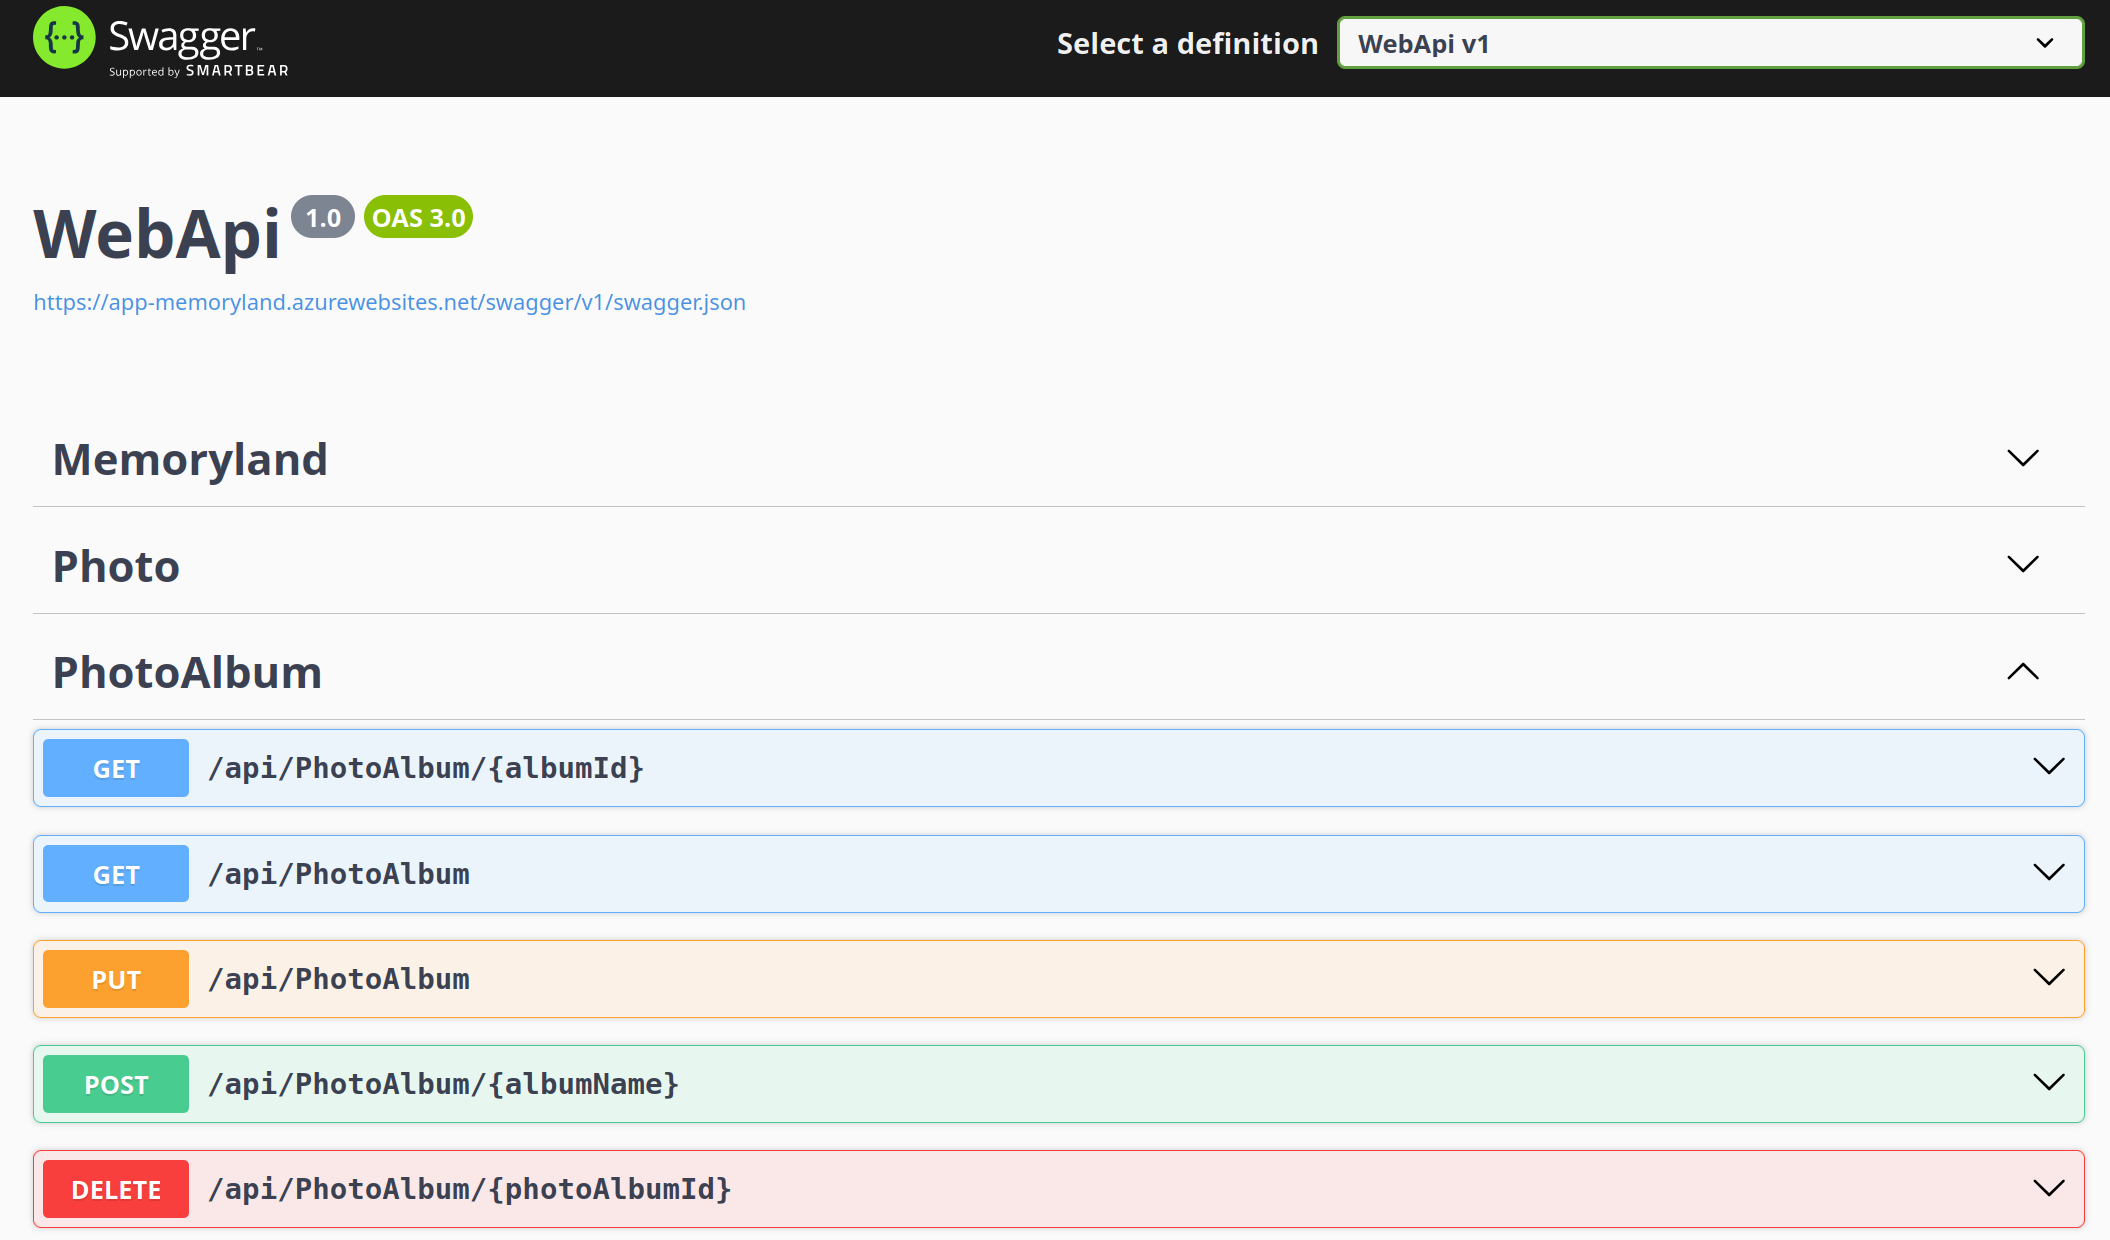
\includegraphics[scale=0.15]{pics/swagger-ui-example.png}
    \caption{Beispiel einer Swagger-UI}
    \label{fig:swagger-ui-example}
\end{figure}

Swagger beinhaltet eine Reihe von Tools, darunter die Swagger UI für interaktive 
API-Dokumentation und Swagger Codegen zur Generierung von Client-Bibliotheken.

Für diese Diplomarbeit wurde OpenAPI genutzt, um eine klare API-Dokumentation bereitzustellen. 
Die Swagger UI (User Interface) insbesondere erleichtert das Testen der API und erleichtert 
es das Frontend an das Backend zu verknüpfen.
\footnote{Alle Informationen zu Swagger und OpenAPI stammen von: \cite{SmartBearSoftware}}

